\documentclass[notitlepage,12pt]{jedm}
%\usepackage[sc,sf,small]{titlesec}
\usepackage[table]{xcolor}
\usepackage{url}
\usepackage{hyperref}
\usepackage{multirow}
\usepackage{graphicx}
\hypersetup{
  colorlinks   = true, %Colours links instead of ugly boxes
  urlcolor     = blue, %Colour for external hyperlinks
  linkcolor    = blue, %Colour of internal links
  citecolor    = blue %Colour of citations
}
\DeclareUnicodeCharacter{202F}{FIX ME!!!!}

%-----------------------------------------------------------------------
% FINAL COPYEDITTED SUBMISSION - UNCOMMENT THIS TO SUPPRESS PAGE NUMBERS
%\pagenumbering{gobble}
%-----------------------------------------------------------------------

\begin{document}

\title{Fighting College Attrition Through Timely Interventions: A Sequential Machine Learning Model}
\date{} %do not delete this, it suppresses insertion of the date

\author{{\large Juan Carlos Apitz}\\California State University Long Beach \\juan.apitz@csulb.edu \and {\large Mahmoud Albawaneh }\\California State University Long Beach \\mahmoud.albawaneh@csulb.edu  \and {\large Janaki Santhiveeran }\\California State University Long Beach \\janaki.s@csulb.edu \and {\large Dhushy Sathianathan }\\California State University Long Beach \\dhushy.sathianathan@csulb.edu}

\maketitle

\begin{abstract}
This is the abstract. It should contain from 100 to 250 words.\\ %Keep \\ for spacing to keywords

{\parindent0pt
\textbf{Keywords:} attrition, machine learning, CatBoost, XGBoost
}
\end{abstract}


\section{Introduction}

\par Attrition, defined as current college students not re-enrolling for a subsequent term, is arguably the most complicated issue facing institutions of higher education (Kim \& Kim, 2018). While it can occur for a variety of reasons, it serves as a detriment to the students who attrit. Not only does attrition delay their academic progress, keeping them from graduating and entering the workforce with a degree, but it disrupts their momentum. When students spend an extended period away from school, they step away from their established academic mindset and may need to readjust when they return to get back on track. For those who attrit and never return, the time and money spent on their education becomes wasted, leaving them to enter the job market with often outstanding debt and no degree to provide opportunities for higher pay. Beyond the students, high levels of attrition can hurt the economy, as taxpayer money, spent with the intention of creating a more educated workforce and society, fails to deliver optimal returns on investment. 

\par From 2020-2021, the U.S. federal government spent \$2.34 billion on college education through various grants and loans (The College Board, 2021) with the intention of making higher education accessible to students from all socioeconomic backgrounds. From 2019-2020, 55\% of students who received baccalaureate degrees graduated with student loan debt (The College Board, 2021). In this context, institutions of higher education have shifted attention away from making college accessible to new students and are focusing instead on combating attrition, in order to increase the number of students who may graduate on time with minimal debt. 

%(Alternate Phrasing: To better understand the variety of factors that contribute to attrition, researchers…) 

\par A variety of factors contribute to attrition. To better understand these factors, researchers have explored academic preparation (Bishop and Bailey, 2021; Bargmann, Thiele, and Kauffeld, 2022), academic performance, and cost of tuition (Bishop and Bailey, 2021), mainly through surveys. However, this type of research remains limited. Rather than studying factors of attrition individually, interactions between predictors must be considered. Using Machine Learning techniques, this study aims to create a model and develop analytical tools to identify students at risk of attrition at California State University at Long Beach. 

\par The California State University (CSU) system is comprised of 23 campuses and is one of two public university systems in California. Looking at first-time students (students who start at a university as first-years with no prior college experience) in the CSU system, only 63.2\% of the Fall 2015 cohort graduated within six years. The rate is lower for Black (49.7\%) and Hispanic/Latino (57.6\%) students. CSU Long Beach has slightly higher rates, with an overall six-year graduation rate of 75.5\% (64.7\% for Black students and 73.7\% for Hispanic/Latino students) for their Fall 2015 cohort (CSU Website). 

\par The analysis in this paper focuses on attrition in the fourth semester ($s_4$), based on socio-demographic variables, pre-entry variables, and academic performance variables available during the first semester ($s_1$), second semester ($s_2$), and third semester ($s_3$). The goal was to create an effective model to estimate the risk of student attrition in each semester. Here, we chose the fourth semester, but the same methodology can be applied to estimate attrition in any given term. 

\par The main analytical approach in this paper was to build a classification model, using state-of-the-art Machine Learning techniques. We evaluated the performance of a variety of algorithms, such as Logistic Regression, Random Forest, CatBoost, XGBoost, and Light Gradient Boosting Machine. Based on performance metrics, the best model was chosen for implementation. In addition to the application of Machine Learning, a key aspect of the study was the development of key engineer features, which enhanced overall analytic performance.    

%%%%%%%%%%%%%%%%%%%%%%%%%%%%%%%%%%%%%%%%%%%%%%%%%%%%%%%%%%%%%%%%%%%%%%%%%%%%%
\section{Related Work}

\par The literature survey in educational data analysis is elaborated on in this section.  The proposed research is based on the earlier theory of student integration (Tinto, 2006), which suggests that students’ dropout is due to their past and current academic performance.  Others believe that student dropout is due to their lack of focus on academic performance and goal engagement (Álvarez-Pérez et al., 2021).  Undecided students tend to drop out or have low GPAs than those with clear educational goals (Pickenpaugh et al., 2022; Swanson, Vaughan, \& Wilkinson (2017).  Several other factors, such as distance between home and school, social and emotional connection, ethnicity, and first-generation status, contribute to college dropout (Álvarez-Pérez et al., 2021; Pickenpaugh et al., 2022).   Some explored roles of financial aid in determining college dropout (Lee et al., 2021).  Existing research on attrition is often survey-driven, surveying students or programs (Álvarez-Pérez et al., 2021).  However, the proposed study is data-driven, an analytical approach using enrollment data from a four-year state university, California State University, Long Beach.   

\par ML is an assuring method for constructing a prognostic model for dropouts and offers early notice to responsible advisors to take preventive measures to help individual students at the risk of dropping out (Bonifro et al., 2020).  In recent years, growing number of researchers used ML classification methods such as LR (Aulck et al., 2016; Aulck, et al., 2019; Chen, Johri, \& Rangwala, 2018; Kemper, 2020), XGB (Aulck et al., 2019; Kiss et al., 2021; Moghimi \& Metzger, 2022; Moreira de Silva et al, 2022), RF (Aulck et al., 2016; Moreira de Silva et al, 2022), NN (Kiss et al., 2021; Moghimi \& Metzger, 2022; Moreira de Silva et al, 2022), SVM (Moghimi \& Metzger, 2022;), DT (Kemper, 2020; Moghimi \& Metzger, 2022) and other algorithms (Aulck et al., 2016; Kiss et al., 2021; Moghimi \& Metzger, 2022; Aulck et al., 2016) to form predictive models.  Other researchers have used ensemble learning and machine learning algorithms (Kemper, 2020) to improve accuracy.   

\par Several studies have employed machine learning algorithms to identify attrition patterns and dropout rates using data from various universities in the USA (Aulck et al., 2016; Aulck et al., 2019; Delen, Topus, \& Eryarsoy, 2020; Moghimi \& Metzger, 2022).  Studies from the USA have reported contrasting results in prediction accuracy.  For example, in a survey of undergraduate students between 1998 and 2006 from the University of Washington (UW), Aulck et al. (2016) used LR, RF, and KNN to predict dropout.  LR emerged as the best model in predicting dropout accurately at 66.59\%, with its AUC for ROC curve score of .729 using a 30\% random test set (Aulck et al., 2016).  In addition, the top five predictors are GPA in Math, English, and Chemistry classes, first-quarter enrollment, and the first year of enrollment, with a predictive accuracy of 54\% (Aulck et al., 2016).  In contrast, using AUC, Chen, Johri, and Rangwala’s (2018) experiment (3) revealed 99.3\% accuracy in predicting dropout by producing an efficient result (F2 = .955) for both LR and ADA models.  However, they implemented several ML methods to predict dropout, including LR, DT, RF, NB, and ADA.  The study used First Time Undergraduates (FTU) using the first six semester data from 12,293 students enrolled between 2009 and 2013 at George Mason University (GMU) (Chen, Johri, \& Rangwala, 2018).  The most significant features such as GPA, enrolled time, and being a young student (age) contributed to student dropout in these best-performing models (Chen, Johri, \& Rangwala, 2018).  The overall dropout rate at the end of the 6th semester was 23.62\% (Chen, Johri, \& Rangwala, 2018).  Similarly, a study using the following data classification techniques, LR, KNN, RF, SVM, and XGB, on the testing set concluded that three models (LR, XGB, \& RF) predicted re-enrollment by 95\% accuracy with AUROC of .88  (Aulck et al., 2019).  ML approaches were implemented using demographic and academic data of reenrolled students (N=61,497) and non-reenrolled students (n=4,563) who did not return for their third semester resulting in a significant data imbalance (Aulck et al., 2019).  Early college performance emerged as the most critical predictor (Aulck et al., 2019).  In a most recent study, Moghimi and Metzger (2022) used academic performance data from UMass using XGB, DT, SVM, BG, and NN to predict persistence rate.  Although XGB performed significantly better, there is an overall reduction in accuracy from the training set to the test set (88\% vs. 82\%) (Moghimi \& Metzger, 2022).  In addition, using the optimized XGB model, Moghimi and Metzger (2022) predicted that the end-of-term GPA, credits taken, and credit total had the most potent effect on dropout.   

\par In a study of 35,021 American citizens from 2006 to 2015 from a University in the USA using BNN, Delen, Topus, and Eryarsoy (2020) had 20\% of freshmen dropouts for not returning during their 3rd semester.  The authors used ElasticNet (EN) for feature selection (Delen, Topus, \& Eryarsoy, 2020).  The results were mixed and showed that the accuracy of the BNN model using AUC (.84 vs. .83) was slightly better in balanced datasets than in the imbalanced datasets. In contrast, sensitivity was much better  (.70 vs. .43) in balanced datasets when 14-15 features were used (Delen, Topus, \& Eryarsoy, 2020).  Receiving a grant, tuition waiver, or scholarship during fall emerged as an essential feature in predicting freshmen dropout along with receiving financial aid, loan, Fall earned hours, GPA, and ethnicity (Delen, Topus, \& Eryarsoy, 2020).   

\par Several researchers from abroad, including Germany (Kemper, 2020), Hungary (Kiss et al., 2021), China (Niyogisubizo et al., 2022), and Portuguese (Moreira de Silva et al., 2022), have effectively implemented ML algorithms to predict dropout.  For instance, Kemper (2020) forecasted student dropout using 2,556 Industrial Engineering students from Germany who graduated and 620 students who had dropped out of Karlsruhe Institute of Technology (KIT) between 2007 and 2012 using LR and DT. Judging by the sensitivity, both LR and DT predicted dropouts better using balanced (86.2\% vs. 89.6\%) than unbalanced (78.5\% vs. 80.7\%) data when the three-semester dataset was trained (Kemper, 2020).  A study using the following data classification techniques, RF, XGB, GB, and FNN on the test set concluded that the stacking ensemble model predicted nearly 93\% of dropouts (Recall = .93). The model is correct for about 93\% (Precision = .93) while predicting students’ dropout in university courses in China by producing an efficient result (F1= .92) (Niyogisubizo et al., 2022).  ML approach was implemented in Python using its popular package scikit-learn (0.24.2), developed by Google (Niyogisubizo et al., 2022).  

\par Moreira de Silva et al. (2022) used only academic grades in a study of student dropouts at a Portugal university.  Moreira de Silva et al. (2022) used RF, XGB, CatBoost, and ANN on the final test set. They concluded that XGB showed the best result, with the XGB model predicting nearly 92\% of dropouts (Recall = .92 Vs. .88).  The model is accurate for about 90\% (RF=88\%) while predicting students’ dropouts by producing an efficient result (F1==.87 Vs. .85) when compared to RF, the next best model. ML approaches were implemented using demographic and academic data of students (N=333) from computer engineering, including dropouts (n=124) and completed (n=207) students leading up to a significant data imbalance (Moreira de Silva et al., 2022).  The most important predictor was age and the number of failures (Moreira de Silva et al., 2022).  Kiss et al. (2021) analyzed students (N=10,196) from a large Hungarian technical university using three ML models: GB, XGB, and ANN. They used student (N=10,196) dropout data from 2013 and 2018, which included graduated students and dropped out.  The models ANN and XGB predicted over 80\% (Recall = .818 vs .808) with an accuracy and AUC scores of over 85\% (ACC=.858 vs .854; AUC = .916 vs. .920) while predicting student dropouts using all available features during 3rd semester with high precision (.863 vs .861).  The model included demographics, high school performance, and university performance data as predictors (Kiss et al., 2021).  

\par Studies presented in this section used data from enrolled students to develop models to predict mostly dropouts.  Some used training sets (Kemper, 2020; Moghimi \& Metzger, 2022) and others used test sets (Aulck et al., 2016; Aulck, et al., 2019; Moghimi \& Metzger, 2022; Moreira de Silva et al, 2022; Niyogisubizo et al., 2022).  Some researchers used unbalanced (For example, Aulck et al., 2019; Delen, Topus, and Eryarsoy, 2020; Kemper, 2020; Moreira de Silva et al., 2022) and balanced datasets (E.g., Delen, Topus, and Eryarsoy, 2020; Kemper, 2020) datasets.  These studies give a basis for using imbalanced datasets in our ML models.   

\par Among the ML algorithms reviewed in this section, LR (Aulck et al., 2016; Aulck et al., 2019; Chen, Johri, \& Rangwala, 2018, Kemper, 2020) and XGB (Aulck et al., 2019; Kiss et al., 2021; Moghimi \& Metzger, 2022; Moreira de Silva et al., 2022) emerged as the best performing models.  RF (Moreira de Silva et al., 2022) and stacking ensemble (Niyogisubizo et al., 2022) performed significantly better in a few studies.  Consequently, the researchers chose mainly these models to predict dropout, and the models were evaluated using the following metrics.    

\par Several types of evaluation metrics, such as accuracy, recall, sensitivity, and precision (Aulck et al., 2019; Delen, Topus, and Eryarsoy, 2020; Kemper, 2020; Niyogisubizo et al., 2022) were reviewed in this literature review.  Some researchers used AUC for the ROC curve score (Aulck et al., 2016; Aulck et al., 2019; Chen, Johri, \& Rangwala, 2018; Delen, Topus, \& Eryarsoy, 2020) in unbalanced datasets.  Among the best performing models reported by the researchers, LR and ADA models reported the highest accuracy of 99.3\% in predicting dropout by producing the most efficient result using data from First Time Undergraduates (FTU) Chen, Johri, and Rangwala’s (2018).  Meantime, Aulck et al. (2016) found out LR had the least accuracy of 72.9\% in predicting dropout by using undergraduate student data.   

\par The ML models reviewed in this section used several features in their predictive models.  Some used demographic data (Delen, Topus, \& Eryarsoy, 2020; Kiss et al., 2021; Moreira de Silva et al., 2022), academic performance (Aulck et al., 2019; Delen, Topus, \& Eryarsoy, 2020; Kiss et al., 2021; Moghimi \& Metzger, 2022; Moreira de Silva et al., 2022), and goal engagement (Moghimi \& Metzger, 2022) features as predictors of dropout.  These studies guided in selecting study features. 

%%%%%%%%%%%%%%%%%%%%%%%%%%%%%%%%%%%%%%%%%%%%%%%%%%%%%%%%%%%%%%%%%%%%%%%%%%%%%
\section{Student Population and Datasets}

\par The population of study in this project consists of CSULB First Year Students (FYS) at the undergraduate level who begin classes during the Fall of each academic year (Fall cohorts). To conduct the analysis we obtained from CSULB's Ofice of Institutional Research a data set consisting of 12,540 student sample records for the Fall cohorts from 2018 to 2020. We classified such records as follows:

\begin{itemize}
\item Input Features:
\subitem{-} Socio-demographic Characteristics
\subitem{-} Pre-entry Academic Performance
\subitem{-} Semester ($s_i$) Academic Performance
\item Response Variable
\subitem{-} Binomial indicator of student enrollment during the \emph{ith} semester
\end{itemize}

\par As mentioned in the Related Work section, attrition research suggests that there are a variety of factors that impact attrition \cite{alvarez2021academic}. The general modeling hypothesis in this work is that a student's demographic characteristics coupled with their academic preparation in high school and sequential performance in college academics are significant factors for attrition \cite{tinto2006research}. In addition, one of the fundamental ideas of this study is that there is a trade-off between the predictive performance and the value of intervention. Predictive performance tends to be lower when sequential modeling is based on data collected early on, for example academic performance data during the first semester in college. However, the sooner students likely to go into attrition are identified, the more time there is available to devise and implement meaningful interventions.



\subsection{Socio-demographic Characteristics}
\par Understanding the impact of socio-demographic factors on attrition is key in informing policy decisions and intervention programs aimed at fighting attrition. The analysis of these student attributes should lead us to ask high level questions regarding the influence of these factors we may uncover in the process. 

\begin{figure}[h!]
\centering
  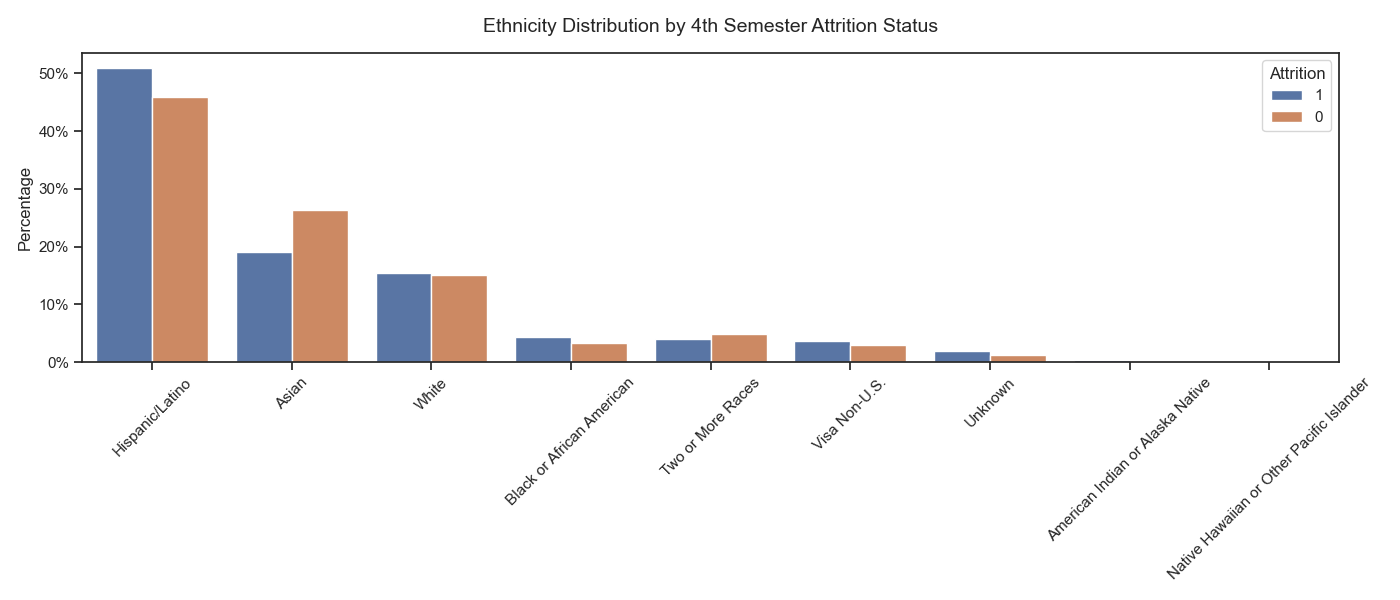
\includegraphics[scale=.45]{ethnicity_attrition_4th_semester.png} 
  \caption{This is the figure's caption.  This is currently a placeholder for the demographics distribution by median zip income.}
  \label{fig:fig1}
\end{figure}

%\subsubsection{Socio-demographic Achievement Gaps}
\par The topic of educational achievement gaps is a field of study on its own right [26]. This area of research highlights the existence of achievements gaps in education but there is no clear agreement as to which socioeconomic factors are true culprits. It is, therefore essential to include and analyze the socio-demographic features of students in order to further understand the social factors that play a role in attrition.  For example, in figure \ref{fig:fig1} we can observe that certain ethnic categories are more likely to go into attrition in the 4th semester. Based on basic exploratory data visualizations, It is difficult to determine to what extent ethnicity and socio-economic circumstances impact attrition outcomes. Thus is is necessary to implement a more rigorous analytical framework such as machine learning in order measure the impact of these variables on attrition. With these facts on hand institutions of higher education will have a unique opportunity to influence the policy agenda and coordination of support to students in order to increase their chances of success.

\subsection{Pre-entry Academic Performance}

\begin{center}
\begin{tabular}{||c | c | c||}
 \hline
 \\ Variables & Attrition & Enrolled \\ [0.5ex]
 \hline
\end{tabular}
\begin{tabular}{||c c c c c c c c c||} 
 \hline
 \\ Pre-Entry Data on Academic Preparation & Attrition & Attrition & Attrition & Attrition & Enrolled & Enrolled & Enrolled & Enrolled \\ [0.5ex] 
 \hline
 \\  & Mean & Std. Dev & Min & Max & Mean & Std. Dev & Min & Max  \\
 \hline
 HS: Overall GPA & 3.51 & 0.39 & 2.56 & 4.29 & 3.66 & 0.35 & 2.33 & 4.41 \\
 \hline
 HS: Math GPA & 3.09 & 0.6 & 1 & 4.2 & 3.24 & 0.56 & 1 & 4.3 \\
 \hline
 HS: English GPA & 3.38 & 0.47 & 1.5 & 4.25 & 3.54 & 0.44 & 1.38 & 4.5 \\ [1ex] 
 \hline
\end{tabular}
\end{center}
 

\par Academic performance prior to entry is crucial in identifying students at risk of attrition as soon as students enter the university. Since we only looked at first-time, first-year students, most had little to no college-level education. Instead, high school performance was observed. High school GPA (overall, math, and English) serves as an early indicator of how well students will do in their first term of college. In most cases, this is the only performance metric prior to a student's first semester.

\par Undeclared students are those who have not yet chosen a major. While students can change their major, even after declaring, undeclared students have a less certain career path and lower levels of commitment to any given program. This could be detrimental as it could mean a lower commitment to the university.

\par Finally, any units earned prior to entry was observed, a measure referred to as the pre-entry load index. Since these were first-time students, this mostly includes college units earned, if any, while the students were in high school, including AP credits or classes taken as transitory students (students not enrolled in a specific program) at colleges or universities. While the pre-entry load index is expected to be very low for first-time students, there may be differences in attrition tendencies between students who took classes prior to college and those who did not.

\subsection{Semester ($s_i$) Academic Performance}

\par In addition to socio-demographic and pre-entry academic performance factors, we include semester by semester college academic performance. According to the theory of academic integration \cite{tinto2006research}, student attrition is due to their past and current academic performance. As students progress through their academic programs each semester, those students who perform adequately, all other circumstances being equal, should have no academic barriers that prevent them form continuing, if they choose to do so. 

\par On the other hand, students who struggle academically at some point will find it difficult to continue and may be prevented by their institutions from re-enrolling in future semesters. For example, at CSULB students must maintain a GPA of at least 2.0 in order to be allowed to matriculate in subsequent semesters. If students fail to maintain a 2.0 GPA by the end of the semester, they receive a warning and must bring their GPA to the required level in the following semester. Failure to do so disqualifies students from subsequent matriculation. But even if students are not academically disqualified, lower academic performance and low course completion rates tend to correlate with attrition rates.

\par Beyond Grade Point Averages for each term, we consider other academic performance indicators. Some of these metrics are engineered metrics which we discuss in the following sub-sections.

\subsubsection{DFW Rates}

\par DFW Rates refer to the ratio of unsuccessful grade results to total grades in a given semester. Typically these are grades designated by the letters D, F and W, but generally should include any grades that result in the student not earning a credit in a class. At CSULB, in addition to D,F and W grades, we include NC (no-credit), WE (withdrawal due to extenuating circumstances) and WU (unauthorized withdrawal).

\par To calculate DFW rates at the individual student level: \[ DFW_s = \frac{ \# DFW_{si} }{ \# CLASSES_{si}  } \] where the $s$ and $i$ subscripts stand for student and $ith$ semester.

\subsubsection{BCMP Cumulative GPA}
\subsubsection{Load Index}

\begin{table}[h!]
  \caption{This is an example of a table that lists the margins of this template.  Captions should follow the same rules as a figure, except that they are put on top of the table.}\vspace*{1ex}
  \label{tab:1}
  \centering
  \begin{tabular}{| l | l | l | l |}
    \hline
    \multicolumn{1}{|c|}{\textbf{Category}} 
    & \multicolumn{1}{c|}{\textbf{Variable Label}} 
    &  \multicolumn{1}{c|}{\textbf{Description}} 
    &  \multicolumn{1}{c|}{\textbf{Type}} \\
    \hline
    \multirow{5}{6em}{\textbf{Socio-demographic Features}} 
    & Gender & Student is male, female or non-binary & Categorical\\
    & Ethnicity & Student's ethnic category & Categorical \\
    & First Generation & Student is first generation to attend  & Categorical \\
    & Pell Eligibility & Student is Pell eligible & Categorical \\
    & Median Zip Income & Median income of student's zipcode & Numerical \\
    & Local Status & Student is from the CSULB local area & Categorical \\
    \hline
    \multirow{5}{5em}{\textbf{Pre-entry Academic Features}} 
    & HS Overall GPA & Overall HS GPA at entry & Numerical\\
    & HS Math GPA & HS GPA in Math classes & Numerical \\
    & HS English GPA & HS GPA in English classes & Numerical \\
    & Admitted Undeclared & Student was admitted as Undeclared & Categorical \\
    & Load Index Pre-entry & Percentage of units transferred & Engineered \\
    \hline
    \multirow{5}{5em}{\textbf{\emph{ith} Semester Academic Performance Features}} 
    & \emph{ith} Standing Status & Academic standing in \emph{ith} semester & Categorical\\
    & \emph{ith} Cum Major Change  & Major change in \emph{ith} semester & Categorical\\
    & \emph{ith} Cum Summer & Summer units prior to \emph{ith} semester & Integer\\
    & \emph{ith} Cum Winter & Winter units prior to \emph{ith} semester & Integer\\
    & \emph{ith} Cum Completion Rate & \% of units completed to \emph{ith} semester & Numerical\\
    & \emph{ith} Cum DFW Rate & \% of DFW grades \emph{ith} semester & Numerical\\
    & \emph{ith} Cum GPA & Cum GPA end of \emph{ith} semester & Numerical\\
    & \emph{ith} Cum BCMP GPA & Cum BCMP GPA end of \emph{ith} semester & Engineered\\
    & \emph{ith} Load Index Post & Load Index Post end of \emph{ith} semester & Engineered\\
    
    \hline    
  \end{tabular}
  
\end{table}

\section{Machine Learning Methods}
\subsection{Logistic Regression}
\subsection{XGBoost}
\subsection{CatBoost}
\subsection{LGBM}

\section{Results}

\section{Conclusions}
Examples of a figure and a table are given in Figure~\ref{tab:fig1} and Table~\ref{tab:1}.

\begin{figure}[h!]
  \centerline{\fbox{\parbox{.66\textwidth}{\centering \raisebox{0pt}[2cm][2cm]{%
        \begin{tabular}{c}
          \cellcolor{blue!35}{\sf This is a figure}\\
          \cellcolor{blue!25}{\sf And yes, you can use colors!}\\
          \cellcolor{blue!15}{\sf As long as it enhances visibility and understanding}\\
        \end{tabular}
  }}}}
  \caption{This is the figure's caption.  It should be a centered paragraph of width 193mm (7.6in). Font size should be 11pt.}
  \label{tab:fig1}
\end{figure}

%%%%%%%%%%%%%%%%%%%%%%%%%%%%%%%%%%%%%%%%%%%%%%%%%%%%%%%%%%%%%%%%%%%%%%%%%%%%%
\section{Appendices}

Supplementary technical material (e.g., mathematical proofs or descriptions of experimental procedures) should be collected in an appendix at the end of the paper (before the acknowledgements and the references sections).

%%%%%%%%%%%%%%%%%%%%%%%%%%%%%%%%%%%%%%%%%%%%%%%%%%%%%%%%%%%%%%%%%%%%%%%%%%%%%
\section{Footnotes and acknowledgments}

Footnotes should be used sparingly and indicated by consecutive superscript numbers in the text. Material to be footnoted should appear at the bottom of the page on which it is referenced. Acknowledgments and grant numbers should be put into a separate `Acknowledgment' section right before the list of references.

%%%%%%%%%%%%%%%%%%%%%%%%%%%%%%%%%%%%%%%%%%%%%%%%%%%%%%%%%%%%%%%%%%%%%%%%%%%%%
\section{References}

References should follow the ACM standard.  The example provided here uses the \texttt{jedm.cls} class file and \texttt{acmtrans.bst} bib style file.  For example, we could write that \citeN{JEDM:baker2009} published a review on EDM in this journal; other reviews were published later \cite[for eg.]{romero2010educational}. The provided ref.bib file contains examples of virtually every possible citation type.


%%%%%%%%%%%%%%%%%%%%%%%%%%%%%%%%%%%%%%%%%%%%%%%%%%%%%%%%%%%%%%%%%%%%%%%%%%%%%
\section{Supporting materials}

Authors are encouraged to submit the data they use and the analysis code in order to replicate and perform rigorous comparisons across studies.  The data and code can be stored on the \texttt{educationaldatamining.org} site for public reference, or stored privately for reviewing purpose only if required. See the online submission instructions for guidance on using and citing code repositories.


%%%%%%%%%%%%%%%%%%%%%%%%%%%%%%%%%%%%%%%%%%%%%%%%%%%%%%%%%%%%%%%%%%%%%%%%%%%%%
\section{Page numbering and sectioning}

For the manuscript to be reviewed, page number should appear at the bottom of each page.  \textbf{For the final version, they must be taken out as the standard JEDM footer is be added.}

%%%%%%%%%%%%%%%%%%%%%%%%%%%%%%%%%%%%%%%%%%%%%%%%%%%%%%%%%%%%%%%%%%%%%%%%%%%%%
\subsection{Sections and subsections}

Section style should follow the example in this document.

%%%%
\subsubsection{Subsection levels}

There should be no more than three levels of sections.

\paragraph{Fourth level.}

The fourth level should simply have their title in the same font style as those of of subsections, without numbering and at the beginning of a paragraph.

%%%%%%%%%%%%%%%%%%%%%%%%%%%%%%%%%%%%%%%%%%%%%%%%%%%%%%%%%%%%%%%%%%%%%%%%%%%%%
\section{Submission}

The journal prefers PDF format, but can also accommodate most other popular formats.  Care should be taken to embed fonts in the rendered PDF. The provided Word template has a larger filesize because it contains embedded fonts.

Instructions for submitting the papers on the website are at \\
\url{http://jedm.educationaldatamining.org/index.php/JEDM/about/submissions#onlineSubmissions}.  You first need to register and log in to the site.  When registering, you must activate your role as ``author''.

% REMOVE NOCITE OR IT WILL LIST EVERYTHING IN YOUR DATABASE AS A REFERENCE
%\nocite{*}

\bibliographystyle{acmtrans}
\bibliography{./ref}

\end{document}
